\documentclass[12pt,twocolumn]{article}
\usepackage[margin=0.7in]{geometry}
\usepackage{graphicx}
\usepackage{cite}
\linespread{1.5}
                                        
%%%%%%%%%%%%%%%%%%%%%%%%%%%%%%%%%%%%%%%%%%%%%%%%%%%%%%%%%%%%%%%%%%%%%%%%%%%%%%%%%%%%%%%%%%%%%%%%%%%%%%%%%%%%%%%%%%%%%%%%%%%%%%%%%%%%%%%%%%%%%%%%%%%%%%%%%%%%%%%%%%%%%%%%%%%%%%%%%%%%%%%%%%%%%%%%%%%%%%%%
                                        
\begin{document}
\title{Single/Double Slit Experiments}
\author{M. Lane and Alex J. Harsell.}
\date{\today}

\maketitle


\begin{abstract}
Particle wave duality is one of the most perplexing concepts in modern physics. This apparent
paradox seems to defy intuition, which is built upon common experience. In this experiment the
double and single slit experiments are performed one photon at a time. It is shown that a single
photon experiences wave interference in both the single and double slit cases. In this sense the
particle and wave natures of light are shown simultaneously, which motivates the paradox of duality
in an undeniable way.
\end{abstract}

\section{Introduction}

\begin{figure}[h!]
	\centering
	\label{fig:eq}
	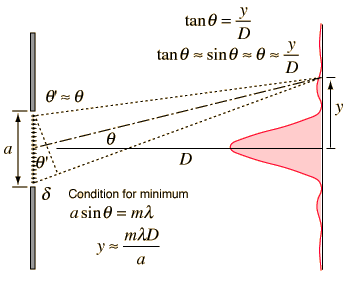
\includegraphics[width=3in]{images/sinslit.png}
	\caption{Replace picture with correct variables or picture in notes}
\end{figure}
For centuries the nature of light has been considerably mysterious. Even the best understanding of light today, in terms of a particle wave duality, remains abhorrent to one’s intuition. The question of whether light is a particle or a wave was posed first, perhaps, through the debate between Sir Isaac Newton and Christian Huygens. Newton advocated a corpuscular theory: he imagined that light was made of discreet particles which propagated in straight lines. Huygens argued an alternative explanation as a wave phenomena. The question was believed to be answered in 1801 when Thomas Young performed the first double slit experiment. He showed that an interference pattern would emerge when light was sent through two crystal, which is clear evidence of wave phenomena.[1] Given Young’s powerful experimental evidence that light is a wave, this view dominated the 1800s. By the turn of the century Faraday and Maxwell had further expanded on the wave interpretation of light by showing that it is a propagating disturbance in an electromagnetic field. The nature of light as a wave phenomena seemed unquestionable. And yet it would be questioned again in 1905 by Albert Einstein. He showed that the photoelectric effect could be most naturally explained by interpreting light as discreet entities, i.e. the photon[2]. Hence it was also shown that light cannot be described simply as waves or as particles. Instead light must be viewed in terms of a particle-wave duality. Hence physics were stuck back the with a concept that defies all previous intuition based on classical mechanics and is not very intuitive today. But as Feynman pointed out, There is one simplification at least... [electrons and photons] are both screwy, but in exactly the same way”[3]. In other words quantum mechanics tells a physicist that all matter is described by the particle-wave duality; hence, by understanding the quirky nature of light the team understands some of the quirkiness of all matter. This paper presents the double slit and single slit diffraction experiments one photon at a time. One shall present strong evidence that the experiment is performed one photon at a time. Further it will be shown that the photons will nevertheless give interference fringes which closely match the predictions of a simple double and single slit interference model. These results superimpose the particle nature of light and the wave nature of light, clearly motivating duality.
There is a simple model which describes classical wave interference for single
and double slits, and can be found in any introductory physics textbook[4]. For single slit
interference one knows that [insert single slit equation]

\begin{figure}[h!]
	\centering
	\label{fig:eq}
	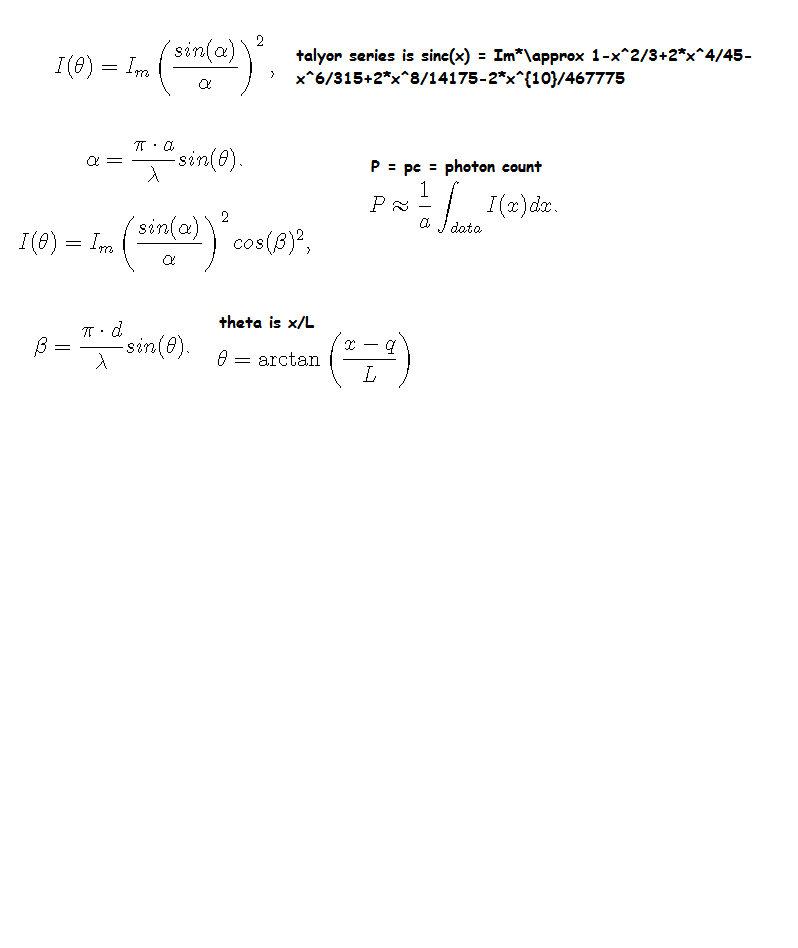
\includegraphics[width=3in]{images/Equations}
	\caption{Equations I nee3d to sort}
\end{figure}

Here I is the central maximum Intensity, a is the slit width, and $\lambda$ is the wavelength of
light. $\theta$ is the angle which is measured relative to a line drawn at the the center of the
single slit, perpendicular to that slit.
For the double slit, one has [insert equation]
Here d is the distance between the centers of the two slits. It is assumed by this model that
each slit has the same width, $a$. $\theta$ is defined in a way that is similar to the $\theta$ in equations
(1) and (2). The only difference being that it is measured relative to a line drawn from the
midpoint of both slits (see Figure \ref{fig:sinslit}).

One notes that $\theta$ is not a variable which was measured directly but measure as a position by trigonometric ratios. The number of photons at a given location was found by allowing light to only pass through a detector slit which was mounted in front of the photomultiplier tube. This detector slit’s location was varied, and measured, with a micrometer drive. Let the distance measured by the
micrometer drive be called x. In order to apply equations [insert] through [fourth insert] to the data collected one can relate $x$ and $\theta$. Let $x_0$ be the position of the central maximum of either a single slit or  double slit plot. The difference $x − x_0$ is shown in \ref{fig:sinslit}. Notice from the figure that [insert equation]
with $L$ is the distance from the double slit to the detector slit. Using this expression we
now have one has a function of $x$. One now has a model for describing wave interference. Next one can develop a method by which one can estimate the total number of photons which pass through a given slit. Consider the plots given in below [insert cross reference]. The goal is to find the total number of photons which pass through the double slit apparatus in one second, which one can call $PC$ (for photon count). Notice the Photon Count in these plots are actually the number of photons which have passed through a detector slit, which happens to be of width $a$. In order to count the total number of photons, imagine that one divides each plot into k rectangles, which are laid side by side; further imagine that the rectangles have width a and height Ik, where Ik is the average height of the curve across the the rectangle. The height of each rectangle then represents the photon count that would be measured if the detector slit were it placed in such a way that it overlapped the rectangle


\section{Method}
\begin{figure}[h!]
	\centering
	\label{fig:setup}
	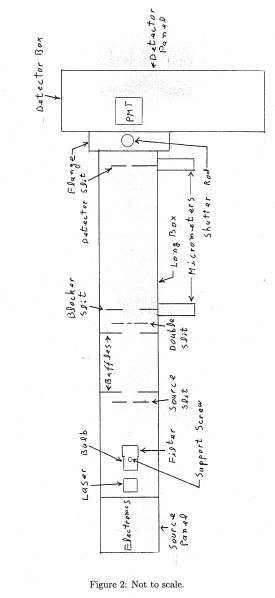
\includegraphics[width=3in]{images/Labphoto1}
	\caption{Results for Two Slit with Laser}
\end{figure}
The experiment was performed using Teach Spin’s “Two-Slit Interference, One Photon at a Time” apparatus (see \ref{fig:setup}). This apparatus consists of a long shaft, one meter long, which is sealed off from outside light sources. On the left side of apparatus is a light bulb whose intensity can be varied. On the end of the light bulb is a filter which only lets through light whose wavelengths are in the green spectrum.   As the light bulb is brought down to low intensities, a red shift in the bulb’s output of wavelengths occurs. Hence the green filter blocks the majority of the light, allowing for very low light intensities. The beam of light passes through a single slit before moving on to the double slit. Just beyond the double slit is a wide slit which can be varied using a micrometer drive. This wide slit can be used to block one light from passing through one or both slits. At far right end of the tube is a detector slit, which can be varied with a second micrometer drive. The light then passes through the detector slit to the Hamamatsu R 212 Photomultiplier Tube. When an incident photon strikes the photomultiplier tube an electron is released. The photomultiplier then multiplies the electron by 105. Each time this electron pulse exceeds a certain threshold, which can be manually adjusted, the photomultiplier gives a clean ttl-level voltage pulse. These pulses signify a discrete photon event, and are sent to the TENMA test equipment 175 MHz universal counter (72-4095). This device counts the number of ttl pulses received per second. However, the device showed significant fluctuations in its measurement. This is believed to be a consequence of having so (relatively) few photons reaching the photomultiplier tube per second. In order to deal with these statistical fluctuations 20 data points per detector slit position were taken in the single slit case and in the double slit case. The average and standard deviations were then calculated, and plotted (see figures 3-5). The team did the photon count with the laser which emitted red light.  The independent variable was the distance that the detector slit was moved in microns, and the dependent variable was the rate of photon incidence in 10 Hz range for convenience of significant figures.


\section{Analysis}

\begin{figure}[h!]
	\centering
	\label{fig:2slit}
	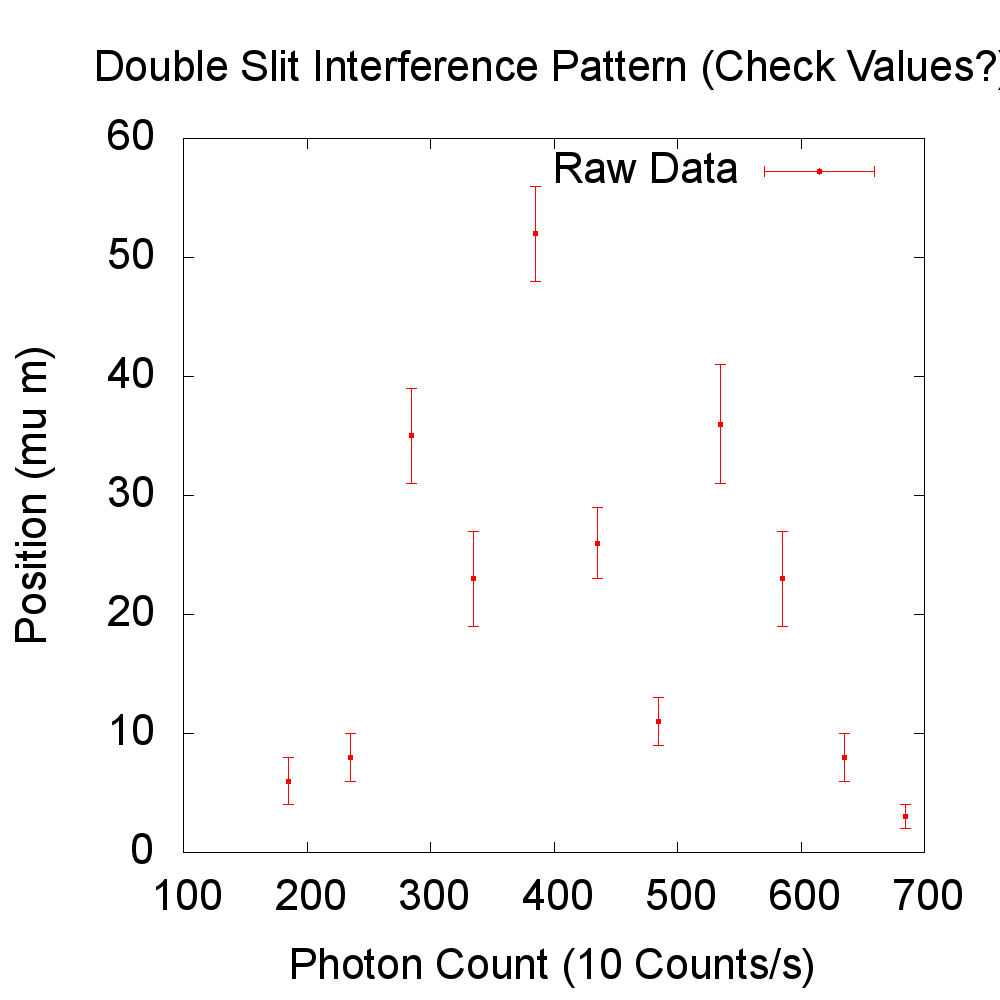
\includegraphics[width=3in]{images/Twoslit}
	\caption{Results for Two Slit with Laser}
\end{figure}
\begin{figure}[h!]
	\centering
	\label{fig:1slit}
	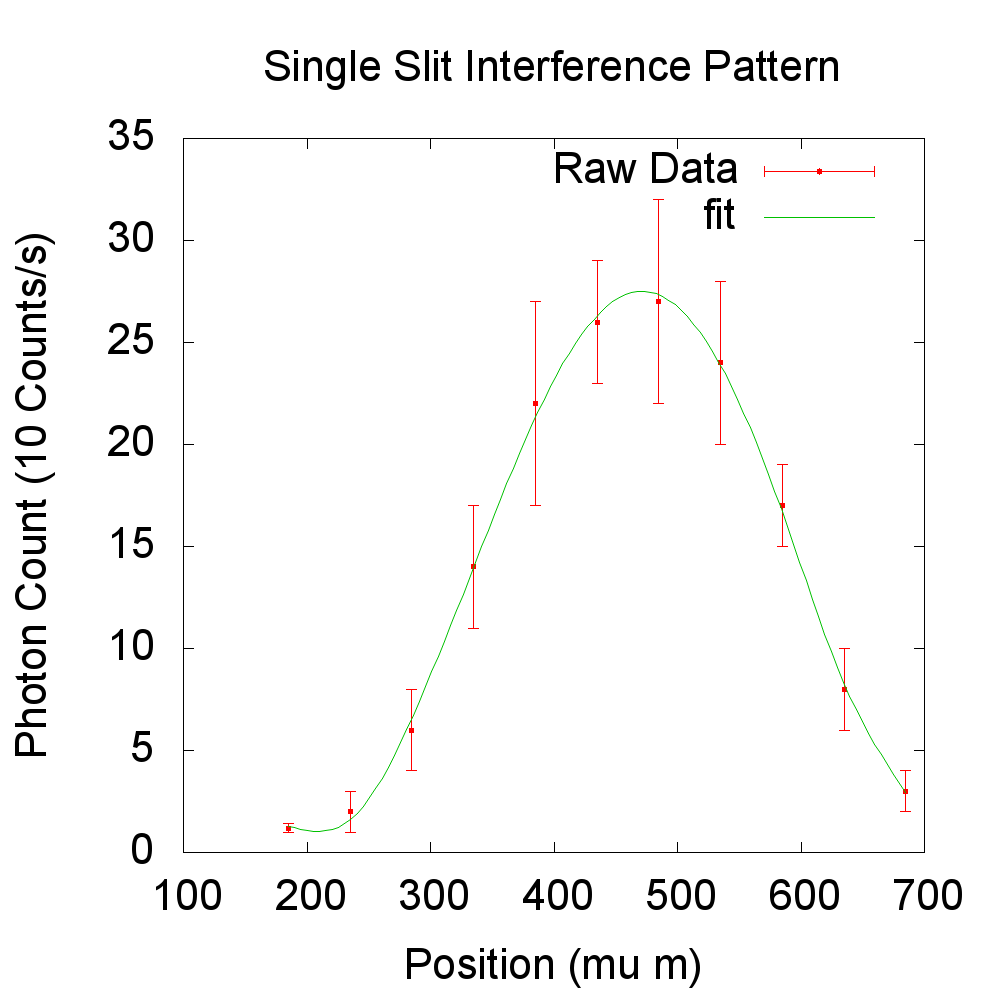
\includegraphics[width=3in]{images/Oneslit}
	\caption{Results for One Slit with Laser}
\end{figure}
Based on the results, One can prove that there is, in fact, only one photon moving through the apparatus
at a time. One can calculate and measure the total number of photons which pass through the two slits using equation in theory.  Here one should approximate (but not by much) by integrating over the interval and taking the Taylor series. I(x) is given by equation (3), with the best fit parameters given in table 1. In the experiment it was found that the count rate was roughly 9000 at peak intensity. However, according to the lab manual of the apparatus the photomultiplier tube is only 4 percent efficient. Hence there are 19000 photons passing through the two slits. Hence one photon passes through the two slits every 1.379 × 10E-6s. Since the distance from the bulb to the detector is L = 9000 meter in length the time it takes a photon to transverse that distance is 9000 s. Observe that the time between photon events is three orders of magnitude greater than time of travel. Hence there is, on average, only one photon moving through the two slits at one time.
Even with only photon in the apparatus at a time, interference fringes are  observed in the time averaged data – strong evidence of the wave nature of light. There are other curiosities in the data. Consider the central maximum of double slit data, which was found to be and is found at the location x = 9000 microns. At this location the intensity for the single slit data is ImL = 9000 photons. One might expect that with discreet events one has that if one doubles the amount of slits through which light can pass then one would double the amount of light observed at a given point. However, this is wrong.  Since the square root of the intensity of light is proportional to the electric field one can attribute this to the fact that when one can have perfectly constructive interference, the magnitude of the resultant electric field vector will be the sum of the magnitudes of the individual vectors.  But this strange additive property is consistent with Quantum Electrodynamics, and hence applies equally well to any other type of matter[5,3]. It is a fundamental property of nature. Upon seeing the above result, one may be curious how all of the photons moving through the apparatus add together when one can switch from single slit interference to double


\nocite{*}
\bibliography{references}
\bibliographystyle{plain}
\end{document}
